\documentclass[12pt,a4paper]{article}

% ─── Page Layout ───────────────────────────────────────────────────────────────
\usepackage[a4paper, margin=0.8in, headheight=14pt]{geometry}

% ─── Fonts (XeLaTeX) ───────────────────────────────────────────────────────────
\usepackage{fontspec}
\usepackage{unicode-math}
\setmainfont{TeX Gyre Pagella}
\setmonofont[Scale=0.88]{TeX Gyre Cursor}
\setmathfont{Latin Modern Math}

% ─── Packages ──────────────────────────────────────────────────────────────────
\usepackage{xcolor}
\usepackage{colortbl}
\usepackage{titlesec}
\usepackage{enumitem}
\usepackage{tabularx}
\usepackage{booktabs}
\usepackage{array}
\usepackage{amsmath}
\usepackage{tikz}
\usetikzlibrary{shapes.geometric, arrows.meta, positioning, calc, fit, decorations.pathreplacing}
\usepackage{tcolorbox}
\tcbuselibrary{skins, breakable}
\usepackage{hyperref}
\usepackage{fancyhdr}
\usepackage{graphicx}
\usepackage{microtype}
\hyphenpenalty=10000
\exhyphenpenalty=10000
\sloppy
\usepackage{caption}
\usepackage{setspace}
\usepackage{multirow}
\usepackage{tocloft}

% ─── Q&A helper ────────────────────────────────────────────────────────────────
\newcommand{\Q}[1]{\textbf{#1}\par\noindent\ignorespaces}

% ─── Colour Palette ────────────────────────────────────────────────────────────
\definecolor{myred}{RGB}{196,30,58}
\definecolor{mydark}{RGB}{30,30,50}
\definecolor{mygreen}{RGB}{14,120,80}
\definecolor{myteal}{RGB}{0,130,140}
\definecolor{myamber}{RGB}{180,100,0}
\definecolor{mypurple}{RGB}{100,30,160}
\definecolor{mygray}{RGB}{246,247,249}
\definecolor{mgframe}{RGB}{180,185,200}
\definecolor{watermark}{RGB}{145,150,170}
\definecolor{hdrred}{RGB}{250,232,235}
\definecolor{hdrgreen}{RGB}{220,244,233}
\definecolor{hdrteal}{RGB}{220,242,244}
\definecolor{hdramber}{RGB}{253,242,215}
\definecolor{hdrpurple}{RGB}{238,228,255}
\definecolor{hdrgray}{RGB}{238,240,245}
\definecolor{rowalt}{RGB}{250,251,253}

% ─── Section Formatting ────────────────────────────────────────────────────────
\titleformat{\section}
  {\large\bfseries\color{myred}}{\thesection.}{0.5em}{}
  [\vspace{1pt}{\color{myred}\rule{\linewidth}{0.8pt}}]
\titleformat{\subsection}
  {\normalsize\bfseries\color{myteal}}{\thesubsection}{0.5em}{}
\titlespacing*{\section}{0pt}{18pt}{7pt}
\titlespacing*{\subsection}{0pt}{11pt}{4pt}

% ─── Paragraph ─────────────────────────────────────────────────────────────────
\setlength{\parindent}{0pt}
\setlength{\parskip}{4pt}

% ─── TOC Styling ───────────────────────────────────────────────────────────────
\renewcommand{\cfttoctitlefont}{\large\bfseries\color{myred}}
\renewcommand{\cftaftertoctitle}{\par\noindent{\color{myred}\rule{\linewidth}{0.8pt}}}
\setlength{\cftbeforetoctitleskip}{0pt}
\setlength{\cftaftertoctitleskip}{6pt}
\renewcommand{\cftsecfont}{\normalsize\bfseries\color{mydark}}
\renewcommand{\cftsecpagefont}{\normalsize\bfseries\color{mydark}}
\renewcommand{\cftsecleader}{\cftdotfill{\cftdotsep}}
\setlength{\cftbeforesecskip}{7pt}
\renewcommand{\cftsubsecfont}{\small\color{mydark}}
\renewcommand{\cftsubsecpagefont}{\small\color{mydark}}
\setlength{\cftbeforesubsecskip}{3pt}
\setlength{\cftsubsecindent}{1.4em}

% ─── Table helpers ─────────────────────────────────────────────────────────────
\renewcommand{\arraystretch}{1.45}
\setlength{\tabcolsep}{6pt}
\arrayrulecolor{mydark}
\newcolumntype{B}[1]{>{\small\bfseries\raggedright\arraybackslash}m{#1}}
\newcolumntype{Y}{>{\small\raggedright\arraybackslash}X}
\renewcommand{\tabularxcolumn}[1]{m{#1}}

% ─── Header / Footer ───────────────────────────────────────────────────────────
\pagestyle{fancy}
\fancyhf{}
\fancyhead[L]{\small\color{myred}\textbf{EC502}\;\color{mydark}--- Computer Architecture}
\fancyhead[R]{\small\color{myteal}\textbf{Module 4 Notes}}
\fancyfoot[C]{\small\color{mydark}\thepage}
\fancyfoot[R]{\small\color{watermark}\textit{\copyright\ Biraj}}
\renewcommand{\headrulewidth}{0.5pt}
\renewcommand{\footrulewidth}{0.3pt}

% ─── Hyperref ──────────────────────────────────────────────────────────────────
\hypersetup{
  colorlinks=true, linkcolor=myteal, urlcolor=myteal,
  pdfauthor={Biraj Sarkar},
  pdftitle={EC502 --- Module 4 Notes}
}

% ─── tcolorbox styles ──────────────────────────────────────────────────────────
\tcbset{
  tikzbox/.style={
    colback=mygray, colframe=mgframe, boxrule=0.6pt, arc=4pt,
    left=8pt, right=8pt, top=6pt, bottom=6pt,
    colbacktitle=mgframe, coltitle=mydark,
    fonttitle=\small\bfseries
  },
  defbox/.style={
    colback=hdrgreen, colframe=mygreen, boxrule=0.8pt, arc=4pt,
    left=9pt, right=9pt, top=6pt, bottom=6pt,
    colbacktitle=mygreen, coltitle=white,
    fonttitle=\small\bfseries
  },
  formulabox/.style={
    colback=hdrteal, colframe=myteal, boxrule=0.8pt, arc=4pt,
    left=9pt, right=9pt, top=7pt, bottom=7pt,
    colbacktitle=myteal, coltitle=white,
    fonttitle=\small\bfseries
  },
  examplebox/.style={
    colback=hdramber, colframe=myamber, boxrule=0.8pt, arc=4pt,
    left=9pt, right=9pt, top=6pt, bottom=6pt,
    colbacktitle=myamber, coltitle=white,
    fonttitle=\small\bfseries
  },
  masonbox/.style={
    colback=hdrpurple, colframe=mypurple, boxrule=0.8pt, arc=4pt,
    left=9pt, right=9pt, top=6pt, bottom=6pt,
    colbacktitle=mypurple, coltitle=white,
    fonttitle=\small\bfseries
  },
  exambox/.style={
    colback=hdrpurple, colframe=mypurple, boxrule=1pt, arc=5pt,
    left=10pt, right=10pt, top=8pt, bottom=8pt,
    colbacktitle=mypurple, coltitle=white,
    fonttitle=\bfseries,
    breakable, title after break={\textbf{Frequently Asked / Viva Questions (contd.)}}}
}
% Make all boxes breakable across pages
\tcbset{breakable}

% ─── TikZ styles ───────────────────────────────────────────────────────────────
\tikzset{
  block/.style={rectangle, draw=myteal, fill=hdrteal,
    text width=2.4cm, align=center, minimum height=0.95cm,
    font=\small, rounded corners=3pt, line width=0.7pt},
  redblock/.style={rectangle, draw=myred, fill=hdrred,
    text width=2.4cm, align=center, minimum height=0.95cm,
    font=\small, rounded corners=3pt, line width=0.7pt},
  netnode/.style={rectangle, draw=myteal, fill=hdrteal,
    text width=1.5cm, align=center, minimum height=0.8cm,
    font=\small, rounded corners=3pt, line width=0.7pt},
  sumjunc/.style={circle, draw=myamber, fill=hdramber,
    minimum size=0.62cm, font=\small, line width=0.8pt},
  snode/.style={circle, draw=mypurple, fill=hdrpurple,
    minimum size=0.55cm, font=\footnotesize, line width=0.7pt},
  arrow/.style={-Stealth, thick, color=mydark},
  redarrow/.style={-Stealth, thick, color=myred},
  line/.style={thick, color=mydark}
}

% ═══════════════════════════════════════════════════════════════════════════════
\begin{document}
% ═══════════════════════════════════════════════════════════════════════════════

\begin{center}
  {\LARGE\bfseries\color{myred} EC502 --- Computer Architecture}\\[5pt]
  {\normalsize\color{mydark} Semester V \quad$\bullet$\quad 3L:0T:0P \quad$\bullet$\quad 3 Credits}\\[3pt]
  {\normalsize\color{myteal}\textbf{Module 4 Exam Notes: Hardwired and Microprogrammed Control}}\\[3pt]
  {\small\color{mydark} CGEC \;$|$\; B.Tech ECE (2023--27) \;$|$\; \textit{Biraj Sarkar}}
\end{center}
\vspace{2pt}
\noindent{\color{myred}\rule{\linewidth}{1.5pt}}
\vspace{2pt}

\hypersetup{linkcolor=mydark}
\tableofcontents
\hypersetup{linkcolor=myteal}
\newpage

\section{Hardwired and Microprogrammed Control}
\begin{tcolorbox}[defbox,title={Control unit and instruction interpretation}]
The control unit converts a machine instruction into an ordered sequence of datapath and memory actions. An instruction is the ISA operation visible to software. A micro-operation is an internal register transfer, ALU operation, shift or similar step implementing it.
\end{tcolorbox}
\subsection{Instruction sequencing on a single bus}
Assume byte addresses, four-byte instructions, a single internal bus, an ALU input latch $Y$, an ALU result latch $Z_{\rm ALU}$ and an independent memory data path to the MDR. A memory-ready signal means read data can now be latched. Transfers on the internal bus and independent local operations may share a cycle only if their signals do not conflict.
\par\vspace{6pt}\noindent
\begin{tabularx}{\linewidth}{|B{2.5cm}|Y|Y|}\hline
Phase & Register transfers & Decision or completion \\ \hline
$F_0$ & $\mathrm{MAR}\leftarrow\mathrm{PC}$ and $Z_{\rm ALU}\leftarrow\mathrm{PC}+4$ from the same bus value using a constant ALU input. & Prepare read and sequential PC. \\ \hline
$F_1$ & $\mathrm{PC}\leftarrow Z_{\rm ALU}$ and request instruction read through MAR. & Hold request until memory ready. MDR latches read data on the ready edge. Rewriting the same PC while waiting is harmless in this model. \\ \hline
$F_2$ & $\mathrm{IR}\leftarrow\mathrm{MDR}$. & The instruction is now available to decode. \\ \hline
Decode & Test opcode and addressing mode. & Dispatch to the corresponding execution routine or state. \\ \hline
$A_0,A_1,A_2$ & For \texttt{ADD R3,R1,R2}: $Y\leftarrow R_1$, then $Z_{\rm ALU}\leftarrow Y+R_2$, then $R_3\leftarrow Z_{\rm ALU}$. & Update flags as specified by the ISA. Return to fetch unless another event is accepted. \\ \hline
\end{tabularx}

\begin{itemize}[leftmargin=*,itemsep=3pt]
\item \textbf{Memory operand.} Compute the effective address, load MAR, issue read, wait, and route MDR to the ALU or a destination. A memory-indirect addressing mode first reads a pointer and uses that pointer for a second memory access.
\item \textbf{Branch.} For a taken PC-relative branch in this model, add the sign-extended, correctly scaled displacement to the sequential PC. Select this target instead of the sequential address.
\item \textbf{Interrupt.} At an instruction boundary in a simple precise model, save the resume PC and required status, then select a handler address. Interrupt return restores the state needed to resume.
\end{itemize}

\subsection{Design a hardwired CPU controller}
\begin{tcolorbox}[defbox,title={Hardwired control}]
A hardwired controller generates control signals using a finite-state machine (FSM) and logic gates or programmable logic. Combinational logic decodes state, opcode and conditions. State registers hold the current step.
\end{tcolorbox}

\begin{enumerate}[leftmargin=*,itemsep=3pt]
\item \textbf{List operations.} Write the required RTL first. Separate any transfers that compete for the bus or depend on data produced only at an edge.
\item \textbf{Choose states and transitions.} Use a fixed sequence counter and decoded timing pulses for simple straight-line sequences. Use an FSM for variable paths involving memory wait, condition flags or instruction-dependent cycle counts.
\item \textbf{Write outputs.} A Moore output depends on state; a Mealy output can also depend on current inputs. For the fetch above, assert \texttt{PCout} in $F_0$, \texttt{IRin} in $F_2$, and read request in $F_1$. Assert MDR latch enable when $F_1$ and ready are both true.
\item \textbf{Implement and check.} Encode states using binary or one-hot encoding, derive next-state and output logic, and implement with gates, decoders or a programmable logic array (PLA). Check reset, memory wait, branch conditions, and mutual exclusion of bus drivers.
\end{enumerate}
\begin{tcolorbox}[tikzbox,title={Hardwired control inputs, state and outputs},unbreakable]
\centering
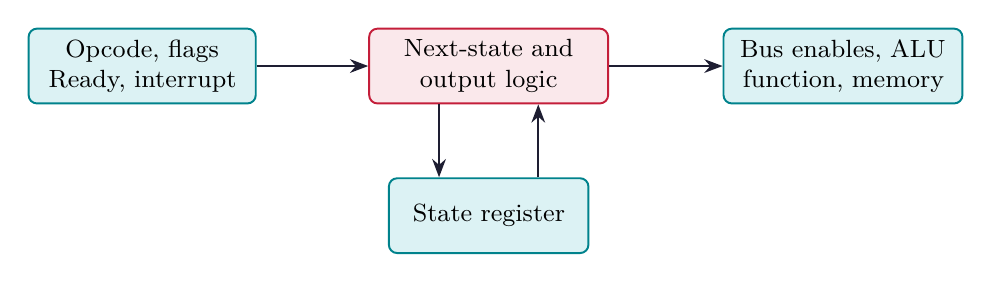
\begin{tikzpicture}[font=\small]
\node[block,text width=2.65cm] (i) at (0,0) {Opcode, flags\\Ready, interrupt};
\node[redblock,text width=2.8cm] (l) at (4.4,0) {Next-state and\\output logic};
\node[block,text width=2.8cm] (o) at (8.9,0) {Bus enables, ALU\\function, memory};
\node[block,text width=2.3cm] (s) at (4.4,-1.9) {State register};
\draw[arrow] (i.east)--(l.west);
\draw[arrow] (l.east)--(o.west);
\draw[arrow] ($(l.south)+(-.63,0)$)--($(s.north)+(-.63,0)$);
\draw[arrow] ($(s.north)+(.63,0)$)--($(l.south)+(.63,0)$);
\end{tikzpicture}
\end{tcolorbox}

\begin{tcolorbox}[examplebox,title={Derive a state equation with a memory wait}]
Use one-hot state bits $F_0,F_1,F_2$ and ready input $M$. Fetch enters $F_1$ from $F_0$. It stays there while not ready, and enters $F_2$ on ready.
\[
 F_1^{+}=F_0+F_1\overline M,\qquad
 F_2^{+}=F_1M,\qquad
 \mathrm{MDRin}=F_1M .
\]
Here $+$ is Boolean OR and superscript $+$ denotes the next stored state. In a one-hot design the reset path establishes one valid starting state. Require the readiness input to obey the interface timing or synchronise it before use.
\end{tcolorbox}

\section{Microprogrammed CPU Control}
\begin{tcolorbox}[defbox,title={Microinstruction and control store}]
A microinstruction holds control actions for a microcycle and information used to choose the next microaddress. A microprogram in a control store implements an ISA instruction or a shared routine such as fetch. The micro-PC addresses the control store, while the ISA PC addresses program memory.
\end{tcolorbox}

\begin{tcolorbox}[tikzbox,title={Microprogrammed controller},unbreakable]
\centering
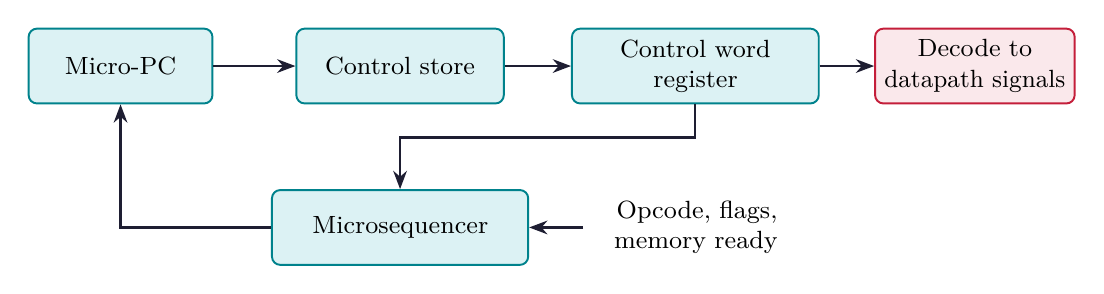
\begin{tikzpicture}[font=\small]
\node[block,text width=2.1cm] (pc) at (0,0) {Micro-PC};
\node[block,text width=2.4cm] (store) at (3.55,0) {Control store};
\node[block,text width=2.90cm] (mir) at (7.3,0) {Control word\\register};
\node[redblock,text width=2.3cm] (out) at (10.85,0) {Decode to\\datapath signals};
\node[block,text width=3.02cm] (seq) at (3.55,-2.05) {Microsequencer};
\node[align=center,text width=2.6cm] (cond) at (7.3,-2.05) {Opcode, flags,\\memory ready};
\draw[arrow] (pc.east)--(store.west);
\draw[arrow] (store.east)--(mir.west);
\draw[arrow] (mir.east)--(out.west);
\draw[arrow] (mir.south)--++(0,-.42)-|(seq.north);
\draw[arrow] (cond.west)--(seq.east);
\draw[arrow] (seq.west)-|(pc.south);
\end{tikzpicture}
\end{tcolorbox}

\subsection{Sequencer, dispatch and example microprogram}
\begin{itemize}[leftmargin=*,itemsep=3pt]
\item \textbf{Fetch microinstruction.} Address the control store with the micro-PC and latch the control word in the microinstruction register (MIR), where the design uses a separate latch.
\item \textbf{Execute micro-operations.} Direct signal bits or decoded fields select register enables, ALU operation and memory controls.
\item \textbf{Select next address.} Choose increment, explicit target, conditional target, opcode dispatch or return from a shared microsubroutine. Opcode mapping supplies an entry address, not a complete execution sequence. Flags may select one of two targets.
\end{itemize}
\par\vspace{6pt}\noindent
\begin{tabularx}{\linewidth}{|B{1.7cm}|Y|Y|}\hline
Address & Control action in the model above & Next address \\ \hline
0 & Perform $F_0$. & 1 \\ \hline
1 & Perform $F_1$, latch MDR only on ready. & If ready then 2, otherwise 1. \\ \hline
2 & Perform $F_2$. & 3 \\ \hline
3 & Decode and dispatch by opcode. & For ADD go to 16, for other operations use their entry points. \\ \hline
16--18 & Schedule $A_0,A_1,A_2$ in order. & Increment through the routine, then jump to 0. \\ \hline
\end{tabularx}

\subsection{Minimise microinstruction size}
\begin{itemize}[leftmargin=*,itemsep=3pt]
\item \textbf{Horizontal.} Allot one bit per independent control line. Wide words can express parallel actions directly and need little control-field decoding.
\item \textbf{Vertical or field encoded.} Encode mutually exclusive actions in a field. Decode the field to select one of them. Separate fields preserve parallelism across groups. Include a no-operation encoding if that group may be idle.
\item \textbf{Sequencing reductions.} Use implicit next-address increment for ordinary steps, reusable micro-routines, and optional branch formats where appropriate. Count address and condition bits explicitly. A $W$-word store needs $\lceil\log_2W\rceil$ address bits.
\end{itemize}
\begin{tcolorbox}[examplebox,title={Compute control-store width}]
Assume eight mutually exclusive source enables, five mutually exclusive ALU functions, and six independent enables. Direct control needs $8+5+6=19$ control bits. Encoding source and ALU with an idle choice needs $\lceil\log_2 9\rceil+\lceil\log_2 6\rceil+6=13$ bits. For a 256-word store with a full next-address field and 2 sequencing bits per word, total width falls from $19+8+2=29$ to $13+8+2=23$ bits. This saves $6(256)=1536$ store bits at the cost of field decoding.
\end{tcolorbox}

\section{Multiplier Control Unit}
\begin{tcolorbox}[defbox,title={Sequential multiplier controller}]
The multiplier controller schedules load, conditional add, shift, decrement and completion. Its status inputs include the multiplier's low bit and the counter-zero condition.
\end{tcolorbox}

For unsigned $n$-bit operands, place the multiplicand in $M$ and the multiplier in $Q$. The accumulator is $A$ and $C$ keeps carry. Use separate states for add and shift to preserve carry. The same state table can drive hardwired gates or a microprogram.
\par\vspace{6pt}\noindent
\begin{tabularx}{\linewidth}{|B{2.6cm}|Y|Y|}\hline
State & Datapath action & Transition \\ \hline
LOAD & Clear $C,A$. Load $M,Q$ and count $n$. & TEST \\ \hline
TEST & Inspect $Q_0$. & If 1, go to ADD. Otherwise go to SHIFT. \\ \hline
ADD & $(C,A)\leftarrow A+M$ using the carry output. & SHIFT \\ \hline
SHIFT & Logical-right-shift $C:A:Q$ and decrement the count. The shifted-in bit at the top is zero. & If the post-decrement count is zero, go to DONE. Otherwise TEST. In a synchronous design test pre-decrement count $=1$ to make this choice at the same edge. \\ \hline
DONE & Assert completion. Read product from $A:Q$. & Idle or LOAD for a new request. \\ \hline
\end{tabularx}

\textbf{Trace.} For $n=3$, $M=3$ and $Q=5$, the three post-shift pairs $(A,Q)$ are $(1,6)$, $(0,7)$ and $(1,7)$. The product is $1\cdot2^3+7=15$. The shifting and count continue even on the iteration that skips ADD.

\newpage
\begin{center}
  {\large\bfseries\color{myred} Quick Revision --- Module 4}\\[3pt]
  {\small\color{mydark} Hardwired and Microprogrammed Control $|$ EC502}
\end{center}
\noindent{\color{myred}\rule{\linewidth}{1.2pt}}
\begin{tcolorbox}[formulabox,title={Key Formulas at a Glance}]
\renewcommand{\arraystretch}{1.35}
\begin{tabularx}{\linewidth}{B{5.0cm}Y}
Fetch address & $\mathrm{MAR}\leftarrow\mathrm{PC}$ \\[3pt]
Simple wait loop & $F_1^{+}=F_0+F_1\overline M$ \\[3pt]
Encoded group & $\lceil\log_2(k+1)\rceil$ bits for $k$ actions plus idle \\[3pt]
Store capacity & Microinstruction width times depth, in bits \\[3pt]
Multiplier termination & Initial count $n$, decrement once per shift \\[3pt]
\end{tabularx}
\end{tcolorbox}
\begin{tcolorbox}[defbox,title={One-Line Definitions}]
\textbf{Micro-operation.} Elementary internal data transfer or computation.\par
\textbf{Control store.} Memory holding the routines that generate CPU control signals.\par
\textbf{Opcode dispatch.} Selection of a microprogram or controller entry state from an opcode.\par
\end{tcolorbox}
\begin{tcolorbox}[exambox,title={Frequently Asked / Viva Questions}]
\begin{enumerate}[topsep=0pt, label=\textbf{Q\arabic*.}, itemsep=5pt]
\item \Q{What is instruction interpretation in a control unit?}
Decoding the instruction and generating the steps that implement its specified operation.
\item \Q{What is the difference between PC and micro-PC?}
PC locates the machine instruction. Micro-PC locates a control-store entry.
\item \Q{Why hold a memory request until ready in this model?}
A fixed cycle count cannot guarantee that memory has produced valid data.
\item \Q{Can two registers drive a single internal bus together?}
The controller normally enables exactly one driver per transfer.
\item \Q{Where do hardwired outputs come from?}
Logic using timing or FSM state, opcode and relevant inputs.
\item \Q{How does a microsequencer handle branches?}
It selects among increment, target, dispatch or return using the microinstruction and conditions.
\item \Q{Where does field encoding save bits?}
Within sets of mutually exclusive actions.
\item \Q{What does a horizontal control word favour?}
Direct selection of many concurrent micro-operations.
\item \Q{When does an unsigned multiplier add the multiplicand?}
When the current low multiplier bit is one.
\item \Q{Why preserve the carry in a multiplier shift?}
It is the high bit of the partial sum and shifts into the accumulator.
\end{enumerate}
\end{tcolorbox}
\begin{tcolorbox}[tikzbox,title={Summary comparison}]
\begin{tabularx}{\linewidth}{|B{4cm}|Y|}\hline
\textbf{Case} & \textbf{What to use} \\ \hline
Hardwired & Control logic implements sequencing directly. Changes can require logic redesign. \\ \hline
Microprogrammed & Control store and sequencer implement steps. Changes can be made in a writable or replaceable store. \\ \hline
Hybrid & Fast common operations may use direct logic, with microcode for more complex sequences. \\ \hline
\end{tabularx}
\end{tcolorbox}
\end{document}
